\documentclass[12pt,a4paper]{article}
	%[fleqn] %%% --to make all equation left-algned--

% \usepackage[utf8]{inputenc}
% \DeclareUnicodeCharacter{1D12A}{\doublesharp}
% \DeclareUnicodeCharacter{2693}{\anchor}
% \usepackage{dingbat}
% \DeclareRobustCommand\dash\unskip\nobreak\thinspace{\textemdash\allowbreak\thinspace\ignorespaces}
\usepackage[top=2in, bottom=1in, left=1in, right=1in]{geometry}
%\usepackage{fullpage}

\usepackage{fancyhdr}\pagestyle{fancy}\rhead{Stephanie Wang}\lhead{EE236B homework 4}

\usepackage{amsmath,amssymb,amsthm,amsfonts,microtype,stmaryrd}
	%{mathtools,wasysym,yhmath}

\usepackage[usenames,dvipsnames]{xcolor}
\newcommand{\blue}[1]{\textcolor{blue}{#1}}
\newcommand{\red}[1]{\textcolor{red}{#1}}
\newcommand{\gray}[1]{\textcolor{gray}{#1}}
\newcommand{\fgreen}[1]{\textcolor{ForestGreen}{#1}}

\usepackage{mdframed}
	%\newtheorem{mdexample}{Example}
	\definecolor{warmgreen}{rgb}{0.8,0.9,0.85}
	% --Example:
	% \begin{center}
	% \begin{minipage}{0.7\textwidth}
	% \begin{mdframed}[backgroundcolor=warmgreen, 
	% skipabove=4pt,skipbelow=4pt,hidealllines=true, 
	% topline=false,leftline=false,middlelinewidth=10pt, 
	% roundcorner=10pt] 
	%%%% --CONTENTS-- %%%%
	% \end{mdframed}\end{minipage}\end{center}	

\usepackage{graphicx} \graphicspath{{}}
	% --Example:
	% \includegraphics[scale=0.5]{picture name}
%\usepackage{caption} %%% --some awful package to make caption...

\usepackage{hyperref}\hypersetup{linktocpage,colorlinks}\hypersetup{citecolor=black,filecolor=black,linkcolor=black,urlcolor=blue,breaklinks=true}

%%% --Text Fonts
%\usepackage{times} %%% --Times New Roman for LaTeX
%\usepackage{fontspec}\setmainfont{Times New Roman} %%% --Times New Roman; XeLaTeX only

%%% --Math Fonts
\renewcommand{\v}[1]{\ifmmode\mathbf{#1}\fi}
%\renewcommand{\mbf}[1]{\mathbf{#1}} %%% --vector
%\newcommand{\ca}[1]{\mathcal{#1}} %%% --"bigO"
%\newcommand{\bb}[1]{\mathbb{#1}} %%% --"Natural, Real numbers"
%\newcommand{\rom}[1]{\romannumeral{#1}} %%% --Roman numbers

%%% --Quick Arrows
\newcommand{\ra}[1]{\ifnum #1=1\rightarrow\fi\ifnum #1=2\Rightarrow\fi\ifnum #1=3\Rrightarrow\fi\ifnum #1=4\rightrightarrows\fi\ifnum #1=5\rightleftarrows\fi\ifnum #1=6\mapsto\fi\ifnum #1=7\iffalse\fi\fi\ifnum #1=8\twoheadrightarrow\fi\ifnum #1=9\rightharpoonup\fi\ifnum #1=0\rightharpoondown\fi}

%\newcommand{\la}[1]{\ifnum #1=1\leftarrow\fi\ifnum #1=2\Leftarrow\fi\ifnum #1=3\Lleftarrow\fi\ifnum #1=4\leftleftarrows\fi\ifnum #1=5\rightleftarrows\fi\ifnum #1=6\mapsfrom\ifnum #1=7\iffalse\fi\fi\ifnum #1=8\twoheadleftarrow\fi\ifnum #1=9\leftharpoonup\fi\ifnum #1=0\leftharpoondown\fi}

%\newcommand{\ua}[1]{\ifnum #1=1\uparrow\fi\ifnum #1=2\Uparrow\fi}
%\newcommand{\da}[1]{\ifnum #1=1\downarrow\fi\ifnum #1=2\Downarrow\fi}

%%% --Special Editor Config
\renewcommand{\ni}{\noindent}
\newcommand{\onum}[1]{\raisebox{.5pt}{\textcircled{\raisebox{-1pt} {#1}}}}

\newcommand{\claim}[1]{\underline{``{#1}":}}

\renewcommand{\l}{\left}\renewcommand{\r}{\right}

\newcommand{\casebrak}[2]{\left \{ \begin{array}{l} {#1}\\{#2} \end{array} \right.}
%\newcommand{\ttm}[4]{\l[\begin{array}{cc}{#1}&{#2}\\{#3}&{#4}\end{array}\r]} %two-by-two-matrix
%\newcommand{\tv}[2]{\l[\begin{array}{c}{#1}\\{#2}\end{array}\r]}

\def\dps{\displaystyle}

\let\italiccorrection=\/
\def\/{\ifmmode\expandafter\frac\else\italiccorrection\fi}


%%% --General Math Symbols
\def\bc{\because}
\def\tf{\therefore}

%%% --Frequently used OPERATORS shorthand
\newcommand{\INT}[2]{\int_{#1}^{#2}}
% \newcommand{\UPINT}{\bar\int}
% \newcommand{\UPINTRd}{\overline{\int_{\bb R ^d}}}
\newcommand{\SUM}[2]{\sum\limits_{#1}^{#2}}
\newcommand{\PROD}[2]{\prod\limits_{#1}^{#2}}
\newcommand{\CUP}[2]{\bigcup\limits_{#1}^{#2}}
\newcommand{\CAP}[2]{\bigcap\limits_{#1}^{#2}}
% \newcommand{\SUP}[1]{\sup\limits_{#1}}
% \newcommand{\INF}[1]{\inf\limits_{#1}}
\DeclareMathOperator*{\argmin}{arg\,min}
\DeclareMathOperator*{\argmax}{arg\,max}
\newcommand{\pd}[2]{\frac{\partial{#1}}{\partial{#2}}}
\def\tr{\text{tr}}

\renewcommand{\o}{\circ}
\newcommand{\x}{\times}
\newcommand{\ox}{\otimes}

\newcommand\ie{{\it i.e. }}
\newcommand\wrt{{w.r.t. }}
\newcommand\dom{\mathbf{dom\:}}

%%% --Frequently used VARIABLES shorthand
\def\R{\ifmmode\mathbb R\fi}
\def\N{\ifmmode\mathbb N\fi}
\renewcommand{\O}{\mathcal{O}}

\newcommand{\dt}{\Delta t}
\def\vA{\mathbf{A}}
\def\vB{\mathbf{B}}\def\cB{\mathcal{B}}
\def\vC{\mathbf{C}}
\def\vD{\mathbf{D}}
\def\vE{\mathbf{E}}
\def\vF{\mathbf{F}}\def\tvF{\tilde{\mathbf{F}}}
\def\vG{\mathbf{G}}
\def\vH{\mathbf{H}}
\def\vI{\mathbf{I}}\def\cI{\mathcal{I}}
\def\vJ{\mathbf{J}}
\def\vK{\mathbf{K}}
\def\vL{\mathbf{L}}\def\cL{\mathcal{L}}
\def\vM{\mathbf{M}}
\def\vN{\mathbf{N}}\def\cN{\mathcal{N}}
\def\vO{\mathbf{O}}
\def\vP{\mathbf{P}}
\def\vQ{\mathbf{Q}}
\def\vR{\mathbf{R}}
\def\vS{\mathbf{S}}
\def\vT{\mathbf{T}}
\def\vU{\mathbf{U}}
\def\vV{\mathbf{V}}
\def\vW{\mathbf{W}}
\def\vX{\mathbf{X}}
\def\vY{\mathbf{Y}}
\def\vZ{\mathbf{Z}}

\def\va{\mathbf{a}}
\def\vb{\mathbf{b}}
\def\vc{\mathbf{c}}
\def\vd{\mathbf{d}}
\def\ve{\mathbf{e}}
\def\vf{\mathbf{f}}
\def\vg{\mathbf{g}}
\def\vh{\mathbf{h}}
\def\vi{\mathbf{i}}
\def\vj{\mathbf{j}}
\def\vk{\mathbf{k}}
\def\vl{\mathbf{l}}
\def\vm{\mathbf{m}}
\def\vn{\mathbf{n}}
\def\vo{\mathbf{o}}
\def\vp{\mathbf{p}}
\def\vq{\mathbf{q}}
\def\vr{\mathbf{r}}
\def\vs{\mathbf{s}}
\def\vt{\mathbf{t}}
\def\vu{\mathbf{u}}
\def\vv{\mathbf{v}}\def\tvv{\tilde{\mathbf{v}}}
\def\vw{\mathbf{w}}
\def\vx{\mathbf{x}}\def\tvx{\tilde{\mathbf{x}}}
\def\vy{\mathbf{y}}
\def\vz{\mathbf{z}}

%%% --Numerical analysis related
%\newcommand{\nxt}{^{n+1}}
%\newcommand{\pvs}{^{n-1}}
%\newcommand{\hfnxt}{^{n+\frac12}}

%%%%%%%%%%%%%%%%%%%%%%%%%%%%%%%%%%%%%%%%%%%%%%%%%%%%%%%%%%%%%%%%%%%%%%%%%%%%%%%%%%%%%%%%%%%%%%%%%%%%%%%%%%%%%%%%%%%%%%%%%%%%%%%%%%%%%%%%%%%%%%%%%%%%%%%%%%%%%%%%%%%%%%%%%%%%%%%%%%%%%%%%%%%%%%%%%%%%%%
\begin{document}
\subsubsection*{Exercise 3.55 [Boyd \& Vandenberghe, 2004]}
{\it Ans:} (a) Differentiate $f(x) = \INT{-\infty}x e^{-h(t)}dt$ and get
$$f'(x) = e^{-h(x)}, f''(x) = -h'(x) e^{-h(x)}$$
Therefore for $x \in\dom h$, $h'(x) \geq 0$, 
$$f''(x) f(x) = -h'(x)e^{-h(x)}\INT{-\infty}x e^{-h(t)}dt \leq 0 \leq (f'(x))^2$$
 since exponentials and their integrals are always positive. \\
\\
(b) Apply the inequality $h(t) \geq h(x) + h'(x) (t-x)$ to the integral, 
\begin{align*}
\INT{-\infty}x e^{-h(t)}dx &\leq \INT{-\infty}x e^{-h(x)-h'(x)(t-x)}dt \\
& = e^{-h(x)}\INT{-\infty}x e^{-h'(x)(t-x)} dt \\
&= e^{-h(x)} \l(\/1{-h'(x)}\r) \INT{-\infty}0 e^s ds \mbox{ (change of variable with $s = -h'(x)(t-x)$)} \\
&= \frac{e^{-h(x)}}{-h'(x)}  \cdot 1
\end{align*} 
Now that $h'(x) < 0$, we get 
$$f''(x)f(x) \leq -h'(x)e^{-h(x)}\l(\frac{e^{-h(x)}}{-h'(x)}\r)= e^{-2h(x)} = (f'(x))^2$$\qed
\newpage\subsubsection*{Additional Exercise 3.5 [Boyd \& Vandenberghe, 2017]}
{\it Ans:} First observe the objective can be written as an over all maximization among $i \times j$ quotients,
\begin{align*}
f_0(x) = \frac{\max_{i=1,\cdots, m} a_i^T x + b_i}{\min_{j=1, \cdots,p} c_j^Tx + d_j} = \max_{i=1, \cdots, m \atop j = 1, \cdots, p} \frac{a_i^T x + b_i}{c_j^Tx + d_j}
\end{align*}
since for fixed $i_0$ and $j_0$, 
$$\frac{\max_{i=1,\cdots, m} a_i^T x + b_i}{\min_{j=1, \cdots,p} c_j^Tx + d_j} \geq \frac{a_{i_0}^T x + b_{i_0}}{\min_{j=1, \cdots,p} c_j^Tx + d_j} \geq \frac{a_{i_0}^T x + b_{i_0}}{ c_{j_0}^Tx + d_{j_0}}$$
(the reverse inequality follows from the combination of maximizing index of numerator and minimizing index of denominator is within the range of the $i\times j$ index pairs.) Let 
$$y_j = \frac{x}{c_j^Tx + d_j}, z_j = \/1{c_j^Tx + d_j}$$
then the following 2 problems are equivalent (identical trick as in textbook \S 4.3.2),
\begin{align*}
\l\{\begin{array}{cc}
\mbox{minimize}& \displaystyle\frac{a_i^T x + b_i}{c_j^Tx + d_j}\\
\mbox{subject to}& \displaystyle Fx \preceq g
\end{array}\r.	&& \l\{\begin{array}{cc}
\mbox{minimize}& \displaystyle a_i^T y_j + b_i z_j\\
\mbox{subject to}& \displaystyle Fy_j - gz_j \preceq 0
\end{array}\r.
\end{align*}
Therefore, combine them all together, we can get the equivalent LP for the original problem,
$$\l\{\begin{array}{cl}
\mbox{minimize } & \displaystyle t \\
\mbox{subject to } &\displaystyle  a_i^T y_j - b_i z_j \leq t \mbox{, for } i=1, \cdots, m, j = 1, \cdots, p \\
& \displaystyle Fy_j - gz_j \preceq 0 \mbox{, for } j=1, \cdots, p \\
\mbox{with variables } &\displaystyle y_j, z_j, t
\end{array}\r.$$
\qed




\newpage\subsubsection*{Exercise 4.21 [Boyd \& Vandenberghe, 2004]}
{\it Ans:} Here only does part (b). \\
Consider Lagrange multiplier, 
\begin{align*}
c & = \lambda 2A(x^\ast - x_c) \\
x^\ast &= \/1{2\lambda} A^{-1} c + x_c
\end{align*}
(Note that $A\in \vS^n_{++}$ must be invertible. ) Since $x^\ast$ must be on the boundary of the ellipsoid $\{x \mid (x - x_c) ^TA(x - x_c)  \leq 1\}$, 
\begin{align*}
1 &= (x^\ast - x_c) ^TA(x^\ast - x_c)\\
&= \/1{(2\lambda)^2} c^T A^{-1} c
\end{align*}
Solve for $\lambda$, 
$$\lambda = \/12\sqrt{c^T A^{-1} c}$$
and 
$$x^\ast = \/1{\sqrt{c^T A^{-1} c}} A^{-1}c + x_c$$
(Note how the final formula assumes $c\neq 0$. )\qed




\newpage\subsubsection*{Exercise 4.25 [Boyd \& Vandenberghe, 2004]}
{\it Ans:} 
Without loss of generality, first look into the constraint induced by the first ellipsoid; we are looking for $a \in \R^n, b\in R$ such that 
$$a^Tx + b > 0 \mbox{ for } x = P_1 u + q_1 \mbox{ with } \|u\|_2 \leq1$$
or,
$$0 < a^T (P_1 u + q_1) + b = u^T P_1 a + q_1^T a + b$$
Rewrite the inequality we get 
$$-b - q_1^T a < u^T P_1 a \leq \|P_1 a\|_2$$
where the last inequality is from Cauchy's. Combine such inequalities for all ellipsoids, we get the SOCP feasibility problem,
$$\l\{\begin{array}{cl}
\mbox{find } & \dps a, b\\
\mbox{subject to }& \dps -b-q_i^T a \leq \|P_i a\|_2 \mbox{, for } i = 1, \cdots, K \\
&\dps  b+q_i^T a \leq \|P_i a\|_2 \mbox{, for } i = K+1, \cdots, L 
\end{array}\r.$$
\qed



\newpage\subsubsection*{Additional Exercise 7.9 [Boyd \& Vandenberghe, 2017]}
{\it Ans:} (a) It is to show the objective function 
$$g(x) = \max_{k=1,\cdots, N} \|f_k(x) - y_k\|_2$$
is a quasiconvex function. Take $t \in \R$, the $t$-sublevelset
\begin{align*}
\{x \mid g(x) \leq t\} & = \{x \mid \|f_k(x) - y_k\|_2 \leq t, k = 1, \cdots N\}\\
&= \CAP{i=1}N \{x \mid \|f_k(x) - y_k\|_2 \leq t\} \\
&= \CAP{i=1}N \l\{x \mid \l\| \/1{c_k^Tx + d_k} (A_kx+b_k) -y_k\r\|_2 \leq t\r\} \\
&= \CAP{i=1}N \l\{x \mid \l\| (A_kx+b_k) - y_k({c_k^Tx + d_k} )\r\|_2 \leq t({c_k^Tx + d_k} )\r\}
\end{align*}
is the intersection of $N$ convex cones and therefore convex. (Note the assumption $c_k^T x + d >0$ is used in the last equality. )\\ 
\\
(b) Here's the graph of $p^\ast$ and the upper/lower bound during the bisection process. Note the $p^\ast$ curve is missing some parts because some subproblems were infeasible; there was no solution and CVX outputted NaN. 
\begin{center}
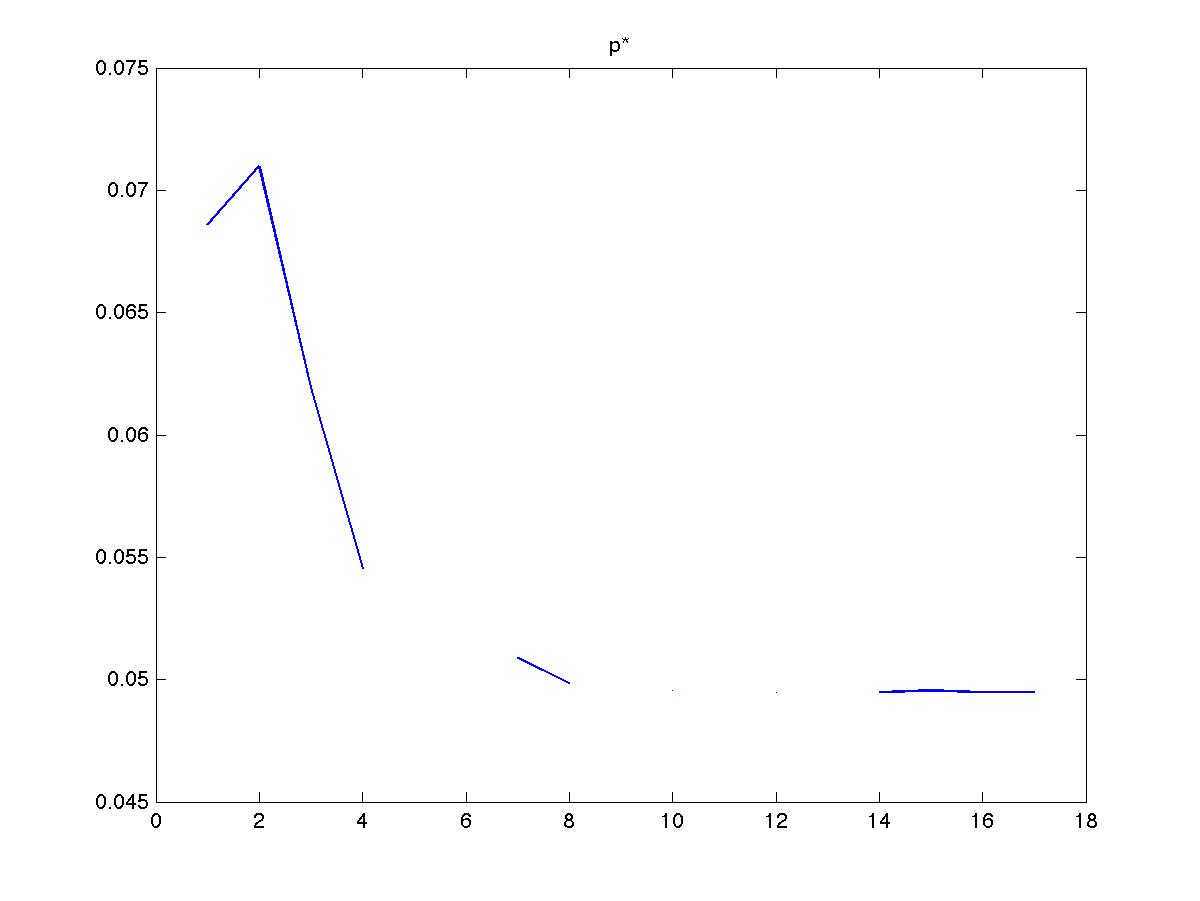
\includegraphics[scale = 0.18]{hw4A79_pstar.jpg}
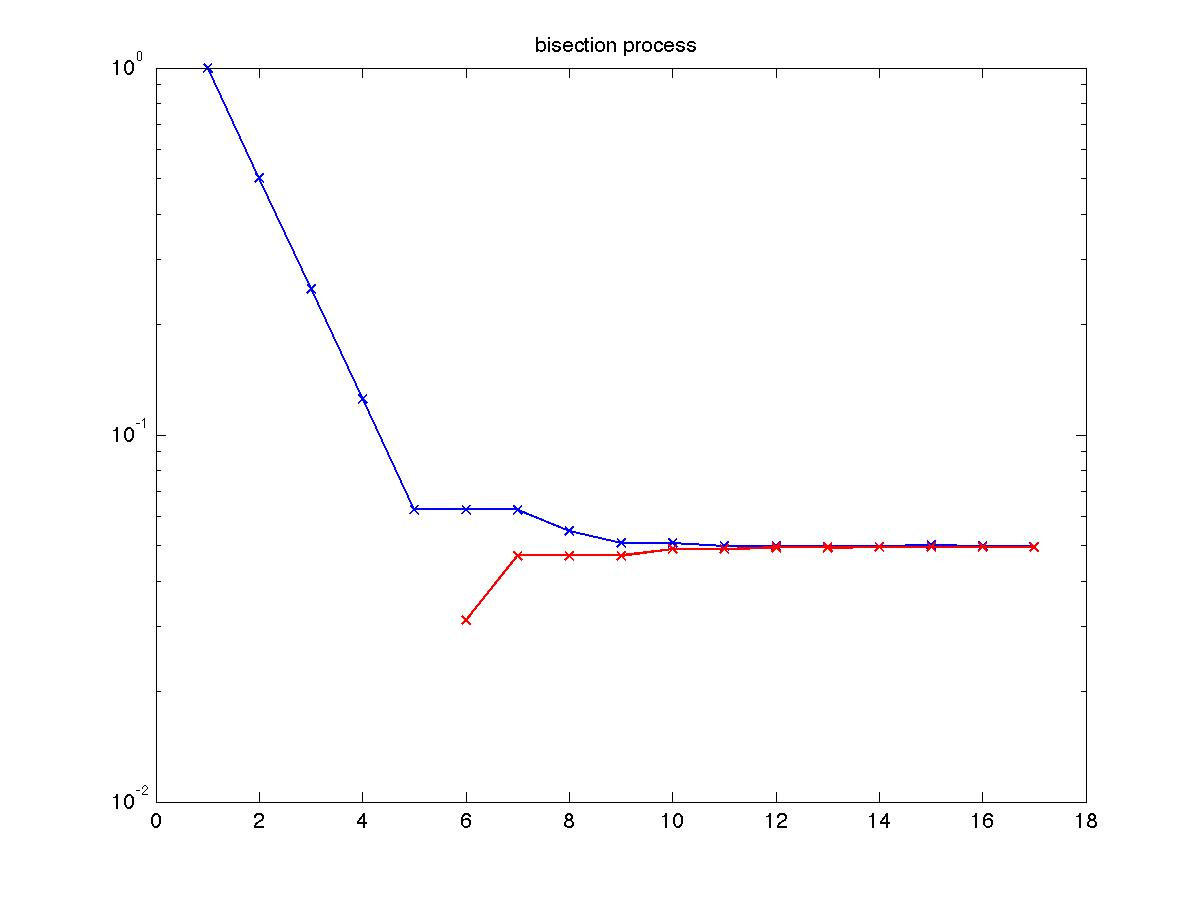
\includegraphics[scale = 0.18]{hw4A79_bisection.jpg}
\end{center}

\begin{verbatim}
%% Problem A7.9
P = zeros(3,4,4);
P(:,:,1) = [1 0 0 0; 0 1 0 0; 0 0 1 0];
P(:,:,2) = [1 0 0 0; 0 0 1 0; 0 -1 0 10];
P(:,:,3) = [1 1 1 -10; -1 1 1 0; -1 -1 1 10];
P(:,:,4) = [0 1 1 0; 0 -1 1 0; -1 0 0 10];

y = zeros(2,4);
y(:,1) = [.98; .93];
y(:,2) = [1.01; 1.01];
y(:,3) = [.95; 1.05];
y(:,4) = [2.04; 0];

f = @(x,k) (P(1:2,:,k)*[x;1])/(P(3,:,k)*[x;1]);
g = @(x) max([norm(f(x,1)-y(:,1)), norm(f(x,2)-y(:,2)), norm(f(x,3)-y(:,3)), norm(f(x,4)-y(:,4))]);


phi_k = @(t,x,k) norm(P(1:2,:,k)*[x;1]-y(:,k)*P(3,:,k)*[x;1]) - t*P(3,:,k)*[x;1];
phi = @(t,x) max([phi_k(t,x,1), phi_k(t,x,2), phi_k(t,x,3), phi_k(t,x,4)]);
TOL = 1e-4;
l = 0;  % objective function is always nonnegative
u = 1;  % random upper bound
num_iter = 0;
while u-l > TOL
    num_iter = num_iter + 1;
    t = 0.5 * (u + l);
    cvx_begin
        variable x(3);
        minimize 1;
        subject to
            phi(t,x) <= 0;
    cvx_end
    p_star(num_iter) = g(x);
    u_data(num_iter) = u;
    l_data(num_iter) = l;
    if cvx_optval == 1
        u = t;
    else
        l = t;
    end
end
h1 = plot(p_star,'LineWidth', 1.1);
title('p*');
saveas(h1,'A79_pstar','jpg');

figure;
semilogy(u_data,'b-x','LineWidth',1.05);
hold on;
h2 = semilogy(l_data,'r-x','LineWidth',1.05);
title('bisection process');
saveas(h2, 'A79_bisection', 'jpg');
\end{verbatim}



\newpage\subsubsection*{Additional Exercise 14.8 [Boyd \& Vandenberghe, 2017]}
{\it Ans:} \\
(a) First write all the constraints in discretized form. The glide slope constraint can be viewed as 
$$[0,0,1] p_k \geq \alpha \l\|\l[\begin{array}{ccc}
1&0&0\\
0&1&0\end{array}\r] p_k\r\|_2 \mbox{ for } k = 0, 1, \cdots, K$$
The position and velocity requires more work. 
\begin{align*}
v_k &= v_{k-1} + \l(\/hm\r) f_{k-1} - hge_3 \\
&= v_{k-2} + \l(\/hm\r) f_{k-2} - hge_3  + \l(\/hm\r) f_{k-1} - hge_3  \\
&= \cdots \\
&= v_1 + \/hm\SUM{i=1}{k-1} f_i - (k-1)hge_3\\
p_{k+1} &= p_k + \/h2 (v_k + v_{k+1}) \\
&= p_{k-1} + \/h2 (v_{k-1}+v_k) + \/h2 (v_k + v_{k+1}) \\
&= \cdots \\
&= p_1 + \/h2 v_1 + h(v_2 + \cdots + v_k) + \/h2 v_{k+1} \\
&= p_1 + \/h2 v_1 + (k-1)h v_1 + h\SUM{j=2}k \l(\/hm\SUM{i=1}{j-1} f_i - (j-1)hge_3\r) + \/h2 v_1 + \/h2 \l(\/hm\SUM{i=1}k f_i - khge_3\r) \\
&= p_1 + khv_1 - \/{k(k+1)}2 h^2 ge_3 + \/{h^2}m\SUM{j=2}k\SUM{i=1}{j-1} f_i + \/{h^2}{2m} \SUM{i=1}k f_i
\end{align*}
Therefore the constraints for touch down is 
\begin{align*}
0 &= v_{K+1}\\
&= v_1 + \/hm\SUM{i=1}{K}f_i - Khge_3 \\
&= v_0 + \/hm f\mathbf 1 - Khge_3 \\
0 &= p_{K+1} \\
&= p_1 + Khv_1 - \/{K(K+1)}2 h^2 ge_3 + \/{h^2}m\SUM{j=2}K\SUM{i=1}{j-1} f_i + \/{h^2}{2m} \SUM{i=1}K f_i \\
&= p_1+ Khv_1 - \/{K(K+1)}2 h^2 ge_3 + \/{h^2}m f\l[\begin{array}{c}
K-1\\
\vdots\\
2\\
1\\
0\end{array}\r] + \/{h^2}{2m}f\mathbf 1  \\
&=p_1+ Khv_1 - \/{K(K+1)}2 h^2 ge_3 + \/{h^2}m f\l[\begin{array}{c}
K-0.5\\
\vdots\\
2.5\\
1.5\\
0.5\end{array}\r]
\end{align*}
where $\mathbf 1 = \l[\begin{array}{c}
1\\
1\\
\vdots\\
1\end{array}\r]$ and $f = [f_1,f_2, \cdots, f_K] \in \R^{3\times K}$. Aside of the constraints, the total fuel use can also be expressed in discretized form since
$$\INT0{T_td} \gamma \|f(t)\|_2 dt \approx \SUM{i=1}K \gamma \|f_k\|_2 h$$
The fuel descent problem can be now formalized
$$\l\{\begin{array}{cl}
\mbox{minimize }& \SUM{i=1}K \gamma h \|f_k\|_2 \\
\mbox{subject to }& v_1 + \/hm\SUM{i=1}{K}f_i - Khge_3 = 0\\
& p_1 + Khv_1 - \/{K(K+1)}2 h^2 ge_3 + \/{h^2}m\SUM{j=2}K\SUM{i=1}{j-1} f_i + \/{h^2}{2m} \SUM{i=1}K f_i  = 0\\
&[0,0,1] p_k \geq \alpha \l\|\l[\begin{array}{ccc}
1&0&0\\
0&1&0\end{array}\r] p_k\r\|_2 \mbox{ for } k = 0, 1, \cdots, K \\
&  p_{k+1} = p_1 + khv_1 - \/{k(k+1)}2 h^2 ge_3 + \/{h^2}m\SUM{j=2}k\SUM{i=1}{j-1} f_i + \/{h^2}{2m} \SUM{i=1}k f_i \mbox{ for } k = 0, 1, \cdots, K 
\end{array}\r.$$
(b) The problem for solving minimum time descent is 
$$\l\{\begin{array}{cl}
\mbox{minimize }& K\\
\mbox{subject to }& v_1 + \/hm\SUM{i=1}{K}f_i - Khge_3 = 0\\
& p_1 + Khv_1 - \/{K(K+1)}2 h^2 ge_3 + \/{h^2}m\SUM{j=2}K\SUM{i=1}{j-1} f_i + \/{h^2}{2m} \SUM{i=1}K f_i  = 0\\
&[0,0,1] p_k \geq \alpha \l\|\l[\begin{array}{ccc}
1&0&0\\
0&1&0\end{array}\r] p_k\r\|_2 \mbox{ for } k = 0, 1, \cdots, K \\
&  p_{k+1} = p_1 + khv_1 - \/{k(k+1)}2 h^2 ge_3 + \/{h^2}m\SUM{j=2}k\SUM{i=1}{j-1} f_i + \/{h^2}{2m} \SUM{i=1}k f_i \mbox{ for } k = 0, 1, \cdots, K 
\end{array}\r.$$
Without any thoughts, this problem can be solved by solving at most $\aleph_0$ (jk, but also not) feasibility problems with $K = 1, 2, \cdots$. \\
\\
(c) \\

\includegraphics{21150888.jpg}

\end{document}